\documentclass[aspectratio=169]{beamer}
\usetheme{Madrid}
\usecolortheme{beaver}
\usefonttheme{serif}
\usepackage{lmodern}

\usepackage[utf8]{inputenc}
\usepackage{graphicx}
\usepackage{pgfplots}
\pgfplotsset{compat=1.18}
\usepackage{amsmath}

% Center frame titles
\setbeamertemplate{frametitle}[default][center]

% Presentation Info
\title[Hydrokinetic Energy]{From Hydroelectricity to Hydrokinetic Energy}
\subtitle{History, Global Need, and Flow-Based Power}
\author[Group 10]{Hamidreza Khalaj Zahrari \and Muhammet Ya\u{g}c\i o\u{g}lu}
\institute[IZTECH]{
    \textbf{Izmir Institute of Technology} \\
    Civil Engineering Department
}
\date{January 5, 2026}

\begin{document}

%--- TITLE PAGE ---
\begin{frame}
    \titlepage
\end{frame}

%--- TOC ---
\begin{frame}{Overview}
    \tableofcontents
\end{frame}

\section{Energy Need \& Current Baseline}

\begin{frame}{Energy Need: Global Electricity Generation Keeps Rising}
    \begin{columns}[T]
        \column{0.42\textwidth}
            \begin{itemize}
                \item Global electricity generation rose from \textbf{11{,}778 TWh} (1990) to \textbf{28{,}927 TWh} (2022).
                \item Demand growth pushes grids to add reliable, low-carbon supply.
            \end{itemize}
            \vspace{0.5em}
            {\scriptsize \textit{Source: Ember data via Our World in Data (2024).}}
        \column{0.58\textwidth}
            \begin{tikzpicture}
                \begin{axis}[
                    width=\textwidth,
                    height=0.55\textheight,
                    ymin=0, ymax=32000,
                    ylabel={TWh},
                    xlabel={Year},
                    xtick={1990,1995,2000,2005,2010,2015,2020,2022},
                    xticklabel style={rotate=45, anchor=east},
                    grid=both,
                    major grid style={line width=.2pt,draw=gray!30},
                    minor grid style={line width=.1pt,draw=gray!15},
                ]
                    \addplot[mark=*, thick, color=blue!70] coordinates {
                        (1990,11778.3)
                        (1995,13150.22)
                        (2000,15278.69)
                        (2005,18133.84)
                        (2010,21264.68)
                        (2015,24014.71)
                        (2020,26742.91)
                        (2022,28926.93)
                    };
                \end{axis}
            \end{tikzpicture}
    \end{columns}
\end{frame}

\begin{frame}{What We Have: Hydropower's Share Is Shrinking}
    \begin{columns}[T]
        \column{0.45\textwidth}
            \begin{itemize}
                \item Hydropower generation increased to \textbf{4{,}321 TWh} in 2022.
                \item Yet its global share fell from \textbf{18.3\%} (1990) to \textbf{14.9\%} (2022).
            \end{itemize}
            \vspace{0.5em}
            {\scriptsize \textit{Source: Ember data via Our World in Data (2024).}}
        \column{0.55\textwidth}
            \begin{tikzpicture}
                \begin{axis}[
                    width=\textwidth,
                    height=0.55\textheight,
                    ybar,
                    ymin=0, ymax=20,
                    ylabel={Share of global electricity (\%)},
                    symbolic x coords={1990,2000,2010,2022},
                    xtick=data,
                    nodes near coords,
                    nodes near coords style={font=\scriptsize, rotate=90, anchor=west},
                    bar width=16pt,
                    grid=both,
                    major grid style={line width=.2pt,draw=gray!30},
                    minor grid style={line width=.1pt,draw=gray!15},
                ]
                    \addplot[fill=red!70] coordinates {
                        (1990,18.33)
                        (2000,17.21)
                        (2010,16.12)
                        (2022,14.94)
                    };
                \end{axis}
            \end{tikzpicture}
    \end{columns}
\end{frame}

\section{Hydropower: History \& Modern Applications}

\begin{frame}{The First Commercial Hydroelectric Plant (1882)}
    \begin{columns}[T]
        \column{0.42\textwidth}
            \begin{itemize}
                \item Appleton, Wisconsin: waterwheel \(\rightarrow\) leather belts \(\rightarrow\) dynamo.
                \item Powered early electric lighting for local buildings.
                \item Lester Pelton later improved turbine efficiency.
            \end{itemize}
            \vspace{0.5em}
            {\scriptsize \textit{Sources: Wikipedia contributors (n.d.-a, n.d.-b).}}
        \column{0.58\textwidth}
            \centering
            \includegraphics[width=\linewidth]{1.png}
            \vspace{0.2em}

            {\scriptsize \textit{Figure 1. The first commercial hydroelectric plant in Appleton, Wisconsin (1882).}}
    \end{columns}
\end{frame}

\begin{frame}{Pumped Storage and Diverse Global Uses}
    \begin{columns}[T]
        \column{0.42\textwidth}
            \begin{itemize}
                \item Pumped storage shifts energy by pumping water uphill during surplus power.
                \item Acts as grid-scale energy storage for daily and weekly balancing.
                \item Run-of-river and tidal barrages expand hydropower with less impoundment.
            \end{itemize}
            \vspace{0.5em}
            {\scriptsize \textit{Sources: Yang \& Jackson (2011); Wikipedia contributors (n.d.-c).}}
        \column{0.58\textwidth}
            \centering
            \includegraphics[width=\linewidth]{2.png}
            \vspace{0.2em}

            {\scriptsize \textit{Figure 2. Pumped storage as a "battery" with other low-impact hydro options.}}
    \end{columns}
\end{frame}

\begin{frame}{Massive Modern Arch-Gravity Dam}
    \begin{columns}[T]
        \column{0.42\textwidth}
            \begin{itemize}
                \item Arch-gravity dams combine weight and arch action to resist water pressure.
                \item Kaplan turbines suit high-flow, low-head rivers common in mega-projects.
                \item Projects provide power, flood control, and irrigation water.
            \end{itemize}
            \vspace{0.5em}
            {\scriptsize \textit{Source: Wikipedia contributors (n.d.-d).}}
        \column{0.58\textwidth}
            \centering
            \includegraphics[width=\linewidth]{3.png}
            \vspace{0.2em}

            {\scriptsize \textit{Figure 3. A modern arch-gravity dam with Kaplan turbine layout.}}
    \end{columns}
\end{frame}

\section{Introducing Hydrokinetic Energy}

\begin{frame}{Introducing Hydrokinetic Energy: Harnessing Flow, Not Fall}
    \begin{columns}[T]
        \column{0.52\textwidth}
            \begin{block}{Hydrokinetic Energy}
                Hydrokinetic energy converts the \textbf{kinetic energy} from flowing water
                (rivers, tides, currents) into electrical power, \textbf{without requiring large dams}
                to create an elevation difference (head).
            \end{block}
            \vspace{0.3em}
            \begin{itemize}
                \item Sits between traditional hydropower and marine energy.
                \item Uses free-flowing water with minimal civil works.
                \item Ideal for canals, straits, and run-of-river corridors.
            \end{itemize}
            \vspace{0.3em}
            {\scriptsize \textit{Source: Khan, Iqbal, \& Quaicoe (2008).}}
        \column{0.48\textwidth}
            \centering
            \includegraphics[width=\linewidth]{w.png}
            \vspace{0.2em}

            {\scriptsize \textit{Figure 4. Hydrokinetic energy: flow-based conversion without dams.}}
    \end{columns}
\end{frame}

\begin{frame}{Power From Moving Water}
    \begin{columns}[T]
        \column{0.48\textwidth}
            \textbf{Kinetic Power Equation}
            \begin{equation*}
                P = \frac{1}{2} \rho A v^3 \eta
            \end{equation*}
            \small
            \begin{itemize}
                \item \(\rho\): water density (\(\approx 1000\,kg/m^3\))
                \item \(A\): rotor area
                \item \(v\): flow velocity
                \item \(\eta\): overall efficiency
            \end{itemize}
            \vspace{0.5em}
            {\scriptsize \textit{Doubling velocity increases power by \(2^3=8\) times.}}
        \column{0.52\textwidth}
            \begin{tikzpicture}
                \begin{axis}[
                    width=\textwidth,
                    height=0.55\textheight,
                    xlabel={Flow velocity (m/s)},
                    ylabel={Power density (kW/m$^2$)},
                    ymin=0, ymax=20,
                    domain=0:3.2,
                    samples=80,
                    grid=both,
                    major grid style={line width=.2pt,draw=gray!30},
                    minor grid style={line width=.1pt,draw=gray!15},
                ]
                    % Assumes rho=1000 kg/m^3, eta=0.4, A=1 m^2
                    \addplot[thick, color=blue!70] {0.5*1000*0.4*x^3/1000};
                \end{axis}
            \end{tikzpicture}
    \end{columns}
\end{frame}

\section{Takeaways}

\begin{frame}{Key Takeaways}
    \begin{itemize}
        \item Global electricity demand keeps growing; firm renewables are critical.
        \item Hydropower output rose, but its global share has declined.
        \item Legacy hydro spans early waterwheels, pumped storage, and mega-dams.
        \item Hydrokinetic systems extend hydropower into low-impact, flow-only sites.
    \end{itemize}
\end{frame}

\begin{frame}[allowframebreaks]{References (APA 7)}
    \small
    Ember. (2024). \textit{Electricity generation by source (TWh)} [Data set]. Our World in Data. \url{https://ourworldindata.org/grapher/electricity-prod-source-stacked.csv}

    Khan, M. J., Iqbal, M. T., \& Quaicoe, J. E. (2008). River current energy conversion systems: Progress, prospects and challenges. \textit{Renewable and Sustainable Energy Reviews, 12}(8), 2177--2193. \url{https://doi.org/10.1016/j.rser.2007.04.016}

    Yang, C.-J., \& Jackson, R. B. (2011). Opportunities and barriers to pumped-hydro energy storage in the United States. \textit{Renewable and Sustainable Energy Reviews, 15}(1), 839--844. \url{https://doi.org/10.1016/j.rser.2010.09.020}

    Wikipedia contributors. (n.d.-a). \textit{Vulcan Street Plant}. In \textit{Wikipedia}. Retrieved January 1, 2026, from \url{https://en.wikipedia.org/wiki/Vulcan_Street_Plant}

    Wikipedia contributors. (n.d.-b). \textit{Pelton wheel}. In \textit{Wikipedia}. Retrieved January 1, 2026, from \url{https://en.wikipedia.org/wiki/Pelton_wheel}

    Wikipedia contributors. (n.d.-c). \textit{Pumped-storage hydroelectricity}. In \textit{Wikipedia}. Retrieved January 1, 2026, from \url{https://en.wikipedia.org/wiki/Pumped-storage_hydroelectricity}

    Wikipedia contributors. (n.d.-d). \textit{Kaplan turbine}. In \textit{Wikipedia}. Retrieved January 1, 2026, from \url{https://en.wikipedia.org/wiki/Kaplan_turbine}
\end{frame}

\end{document}
